%-------------------------------------------------------------------------------
% seq24_patterns_panel
%-------------------------------------------------------------------------------
%
% \file        seq24_patterns_panel.tex
% \library     Documents
% \author      Chris Ahlstrom
% \date        2015-07-19
% \update      2015-08-30
% \version     $Revision$
% \license     $XPC_GPL_LICENSE$
%
%     Provides the concepts.
%
%-------------------------------------------------------------------------------

\section{Patterns Panel}
\label{sec:seq24_patterns_panel}

   \textsl{Seq24} works with the idea of patterns (loops) that are repeated
   all along a song.  One composes and edits small patterns, and combines
   them to create a full song.  This is a powerful way to work, and makes
   one productive within an hour.

   The \textsl{Seq24 Patterns Panel} is the main window of \textsl{Seq24}.
   See \figureref{fig:seq24_main_screen}.
   It is also called the "main window" or the "patterns window".
   It is here one manages a set of patterns
   (see \sectionref{subsubsec:concepts_terms_screen_set}),
   manages the configuration, and opens the pattern or song editors.

   For exposition, we break it into a top panel, a pattern panel, and a
   bottom panel.  Note that the \textsl{Seq24} main menu is discussed in
   \sectionref{sec:seq24_menu}.

\subsection{Patterns / Top Panel}
\label{subsec:seq24_patterns_panel_top}

   The top panel of the Pattern window is simple, consisting of the name of
   the program and a couple of controls.

\begin{figure}[H]
   \centering 
   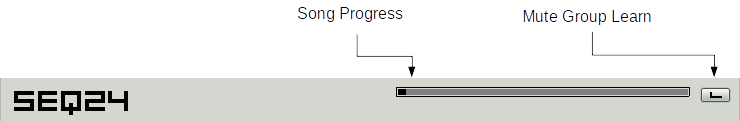
\includegraphics[scale=0.75]{pattern-window-top-panel-items.png}
   \caption{Patterns Panel, Top Panel Items}
   \label{fig:pattern_window_top_panel_items}
\end{figure}

   \begin{enumber}
      \item \textbf{Song Progress}
      \item \textbf{Mute Group Learn}
   \end{enumber}

   \setcounter{ItemCounter}{0}      % Reset the ItemCounter for this list.

   \itempar{Song Progress}{pattern!progress}
   \index{song!progress}
   \index{song!"main time"}
   The \textbf{Song Progress} bar is also known as the "main time" bar.
   This bar shows a number of small black cursors ("pills") that show the
   progress of the song through the various patterns.  For short patterns,
   the progress is fast.  For patterns that last longer, the progress is
   slow.  This field shows that something is going on.  It can also indicate
   the relative lengths of the various patterns.
 
   Note that the individual pattern boxes in the main panel have their own
   moving progress cursor, a tall thin line in each box.  Unfortunately,
   this bar moves along even in patterns that have no events, only meta
   items such as the track name.

   \itempar{Mute Group Learn}{pattern!mute group learn}
   \index{"L" button}
   This button is also known as the "L" button.
   Click this button, and then press a mute-group key
   to store the mute-state of the patterns in that key.

   See the \textbf{File / Options / Keyboard} menu entry to bring up the
   dialog showing the available mute-group keys and the corresponding
   hot-key for the "L" button.

   \index{group!toggle}
	One can toggle the playing status of up to 32 previously
	defined mute/unmute patterns (groups) in the active screen
	set, similar to hardware sequencers.
	This toggling is done either by one of the \textsl{group toggle} keys
	or by a MIDI controller, both assigned in the
   \texttt{~/.seq24rc} file.
	A mute/unmute pattern (group) is stored by holding a
   \index{group!learn}
   \textsl{group learn} key (\texttt{Insert} by default) while pressing the
   corresponding \textsl{group toggle} key.
	There are also keys assigned to turn on/off the group
	functionality.

\subsection{Patterns / Main Panel}
\label{subsec:seq24_patterns_panel_main}

   The main panel of the Patterns window provides a grid of empty boxes,
   each box delimited by brace-like lines at left and right.
   Each filled box represents a loop or pattern.
   One sees only 32 loops at a time in the main panel (but more 32
   loops can be supported by \textsl{Seq24}.
   \index{screen set}
   This group of 32 loops is called a "screen set", as discussed in
   \sectionref{subsubsec:concepts_terms_screen_set}.
   One can switch between sets
   by using the
   \index{keys![}
   \texttt{[} and
   \index{keys!]}
   \texttt{]} keys on the keyboard, or by using
   the spin-widget-driven, labelled \textbf{Set} interface item.
   There are a total of 32 sets, for a total of
   1024 loops/patterns. 

\begin{figure}[H]
   \centering 
   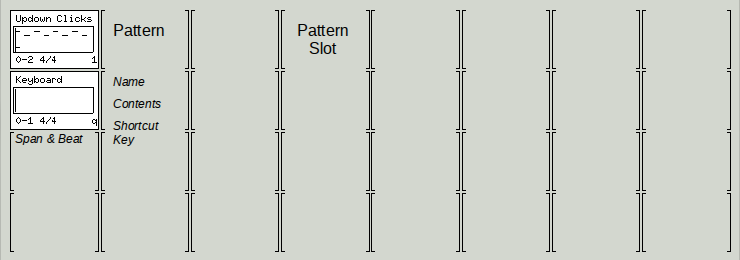
\includegraphics[scale=0.75]{pattern-window-main-panel-items.png}
   \caption{Patterns Panel, Main Panel Items}
   \label{fig:pattern_window_main_panel_items}
\end{figure}

   \begin{enumber}
      \item \textbf{Pattern Slot}
      \item \textbf{Pattern}
   \end{enumber}

\subsubsection{Pattern Slot}
\label{subsubsec:seq24_patterns_pattern_slot}

   \index{pattern!slot}
   An empty box is a slot for a pattern.
   \index{pattern!right click}
   By right-clicking on an empty box one brings up a menu to create
   a new loop, as well as some other operations:

\begin{figure}[H]
   \centering 
   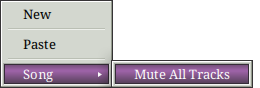
\includegraphics[scale=0.75]{pattern/pattern-empty-right-click-menu.png}
   \caption{Empty Pattern, Right-Click Menu}
   \label{fig:pattern_window_empty_right_click}
\end{figure}

   \begin{enumber}
      \item \textbf{New}
      \item \textbf{Paste}
      \item \textbf{Song / Mute All Tracks}
   \end{enumber}

   \setcounter{ItemCounter}{0}      % Reset the ItemCounter for this list.

   \itempar{New}{pattern!new}
   Creates a new loop or pattern.
   Clicking this menu entry fills in the empty box with an untitled
   pattern, and brings up the Pattern Editor
   so that one can fill in the new pattern.

   \itempar{Paste}{pattern!paste}
   Pastes a loop or pattern that was previously copied.

   \itempar{Song / Mute All Tracks}{pattern!mute all}
   This item is the one item in the \textbf{Song} context menu;
   it mutes all tracks (or loops/patterns).  (We are not clear
   on exactly what it does.  There is no change in visible
   status of any of the patterns in the patterns-panel.)

\subsubsection{Pattern}
\label{subsubsec:seq24_patterns_pattern_filled}

   A filled pattern slot is referred to informally as a pattern.
   A pattern is shown in the Pattern windows as a filled box with the
   following items of information in it:

   \begin{itemize}
      \item \textbf{Name}.
         \index{pattern!name}
         This line contains the name or title of the pattern, to help
         reference it when juggling a number of patters.
      \item \textbf{Contents}.
         \index{pattern!contents}
         The contents of the pattern provide a fairly detailed and
         distinguishable representation of the notes or events in the
         pattern.  Also, when the song is playing, a vertical bar cursor
         tracks the position of the playback of the pattern or loop; it
         returns to the beginning of the box every time that pattern starts
         over again.
         \textbf{Bug:}
         \index{bugs!empty pattern scrolls}
         However, an imported empty pattern will still (needlessly) scroll;
         perhaps such patterns can be marked as inactive.
      \item \textbf{Bus-Channel}.
         \index{pattern!bus-channel}
         This pair of numbers shows the the MIDI buss number, a dash, and
         the MIDI channel number.
         For example, "0-2" means MIDI buss 0, channel 2.
      \item \textbf{Beat}.
         \index{pattern!beat}
         This pair of numbers is the standard time-signature of the pattern,
         such as "4/4" or "3/4".  The first number is the beats-per-measure,
         and the second is the size of the beat, here, a quarter note.
      \item \textbf{Shortcut Key}.
         If the display of shortcut keys is enabled (see
         \sectionref{paragraph:seq24_menu_file_options_keyboard}),
         then the key noted in the lower-right corner of the pattern can be
         pressed to toggle the mute/unmute status of that pattern.
         This action is an alternative to left-clicking on the pattern.
      \item \textbf{Progress Cursor}.
         At the left of each box is a vertical line, waiting for playback to
         start so that it can move through the pattern, again and again.
   \end{itemize}

   \index{pattern!left click}
   Left-clicking on an filled pattern box will toggle the status of the
   pattern between muted (white background) and unmuted (black background).
   If the song is playing via the main window, toggling this status makes
   the pattern stop playing or start playing.  Note that the armed status
   can also be toggled using hot-keys.

   Also note that the pattern boxes will toggle between the muted/unmuted
   states as the music plays, and the pattern is active or inactive at the
   point of playback, if the Song Editor is the active window and was used
   to start the playback.

   \index{pattern!right click}
   By right-clicking on an already-filled box, one brings up a menu
   to allow one to edit a existing one, or perform a few other actions
   specified in the context menu.  Here is that menu:

\begin{figure}[H]
   \centering 
   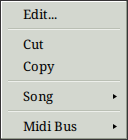
\includegraphics[scale=0.75]{pattern/pattern-right-click-menu.png}
   \caption{Existing Pattern, Right-Click Menu}
   \label{fig:pattern_window_right_click}
\end{figure}

   Here one can choose to edit the pattern, cut and copy the pattern,
   set the MIDI bus/channel, and more.
   One can also clear all performance data for the pattern.
   
   \begin{enumber}
      \item \textbf{Edit...}
      \item \textbf{Cut}
      \item \textbf{Copy}
      \item \textbf{Song/}
      \item \textbf{Midi Bus/}
   \end{enumber}

   \setcounter{ItemCounter}{0}      % Reset the ItemCounter for this list.

   \itempar{Edit}{pattern!edit}
   Edits an existing loop or pattern.
   Clicking this menu entry brings up the Pattern Editor
   so that one can modify the existing pattern.
   See \figureref{fig:pattern_edit_window}.

   \itempar{Cut}{pattern!cut}
   Deletes and copies an existing loop or pattern.

   \textbf{Bug:}
   \index{bugs!pattern cut doesn't work}
   This operation seems to have no effect.  The loop or pattern remains in
   place.

   \itempar{Copy}{pattern!copy}
   Copies an existing loop or pattern.
   The pattern can then be pasted elsewhere in the Patterns panel.
   See \sectionref{subsubsec:seq24_patterns_pattern_slot}.

   \itempar{Song}{pattern!song}
   Clicking this menu entry brings up a small popup menu:

\begin{figure}[H]
   \centering 
   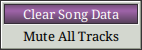
\includegraphics[scale=0.75]{pattern/pattern-menu-song.png}
   \caption{Existing Pattern, Right-Click Menu, Song}
   \label{fig:pattern_window_right_click_song}
\end{figure}

   \begin{enumber}
      \item \textbf{Clear Song Data}
      \item \textbf{Mute All Tracks}
   \end{enumber}

   \setcounter{ItemCounter}{0}      % Reset the ItemCounter for this list.

   \itempar{Clear Song Data}{pattern!clear song data}
   Selecting this filled-box right-click menu item causes that box's
   loop/pattern to be removed from the song.  This means
   that it disappears from the Song Editor window, and so will not
   be played when the song plays.

   \itempar{Mute All Tracks}{pattern!mute all tracks}
   Selecting this filled-box right-click menu item causes...
   TODO.  \index{todo!how mute all tracks works}
   Cannot yet see that this does anything, NEEDS EXPERIMENTATION.

   \itempar{Midi Bus}{pattern!midi bus}
   Selecting this filled-box right-click menu item brings up a list
   of the 16 MIDI output busses that \textsl{Seq24} supports:

\begin{figure}[H]
   \centering 
   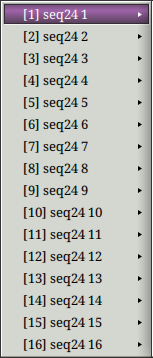
\includegraphics[scale=0.75]{pattern/pattern-menu-midi-bus.png}
   \caption{Existing Pattern, Right-Click Menu, MIDI Output Busses}
   \label{fig:pattern_window_right_click_midi_bus}
\end{figure}

   For each of these buss items, another pop-up menu allows one
   to specify the MIDI output port for that buss:

\begin{figure}[H]
   \centering 
   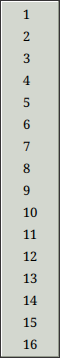
\includegraphics[scale=0.75]{pattern/pattern-menu-midi-bus-numbers.png}
   \caption{Existing Pattern, Right-Click Menu, MIDI Bus Ports}
   \label{fig:pattern_window_right_click_midi_bus_numbers}
\end{figure}

\subsubsection{Pattern Keys and Click}
\label{subsubsec:seq24_patterns_pattern_keys_and_clicks}

   This section recapitulates all the clicks and keys that perform actions
   in the Pattern windows.  Some additional clicks and keys are noted here
   as well.

\paragraph{Pattern Keys}
\label{paragraph:seq24_patterns_pattern_keys}

   \index{keys!pattern toggles}
   For each pattern, hitting its assigned keyboard key will
   also toggle its status between muted/unmuted (armed/unarmed).
   Below is the default grid that is
   mapped to the loops/patterns on the screen set.
   This grid can be changed in the Keyboard options tab, and is
   saved in the \textsl{keyboard-control} section of the
   \texttt{~/.seq24rc} file.

   \begin{verbatim}
     [ 1   ][ 2   ][ 3   ][ 4   ][ 5   ][ 6   ][ 7   ][ 8   ]
     [ q   ][ w   ][ e   ][ r   ][ t   ][ y   ][ u   ][ i   ]
     [ a   ][ s   ][ d   ][ f   ][ g   ][ h   ][ j   ][ k   ]
     [ z   ][ x   ][ c   ][ v   ][ b   ][ n   ][ m   ][ ,   ]
   \end{verbatim}

   These characters are shown in the lower right corner of each
   pattern, as an aid to memory.

   \index{keys![}
   The \texttt{[} and
   \index{keys!]}
   \texttt{]} keys on the keyboard
   switch between sets.

   We're not sure about the functionality of the key sequences involving the 
   \texttt{Alt} key.  The handling of
   \texttt{Alt} is generally taken over by the window manager.

   \index{keys!alt}
   Holding \texttt{Alt} will save the state of playing patterns and restore
   them when \texttt{Alt} is lifted.  Not yet sure exactly what this means.

   \index{keys!left ctrl alt}
   Holding \texttt{Left Ctrl} and \texttt{Alt} at the same time will enable
   one to flip over to new patterns briefly and then flip right back upon
   lifting \texttt{Alt}.  Not yet sure exactly what this means.

   \index{keys!right ctrl}
   \index{queue!temporary}
	Holding \texttt{Right Ctrl} will queue a on/off toggle for a 
	sequence when the loop ends. This is the "temporary queue" functionality.
   Queue also works for mute/unmute 
	patterns (groups); in this case every sequence will toggle 
	its status after its individual loop end. 

   \index{keys!backslash}
   \index{queue!permanent}
   \index{queue!keep queue}
	Pressing the "keep queue" key (by default, the backslash key)
   assigned in the \textsl{~/.seq24rc} file
	activates permanent queue mode until you use the temporary 
	queue function again pressing \texttt{Right Ctrl}. 

\paragraph{Pattern Clicks}
\label{paragraph:seq24_patterns_pattern_Clicks}

   \index{pattern!left click}
   \index{pattern!mute toggle}
   Left-clicking on a pattern-filled box will change its state
   \index{pattern!mute}
   \index{pattern!unmute}
   from muted (white background) to playing (black background) when
   the sequencer is running.

   \index{pattern!left ctrl left click}
   \index{keys!left ctrl}
   Holding down \texttt{Left Ctrl} while selecting a pattern
   with a left click will mute all other patterns and turn on the selected
   pattern.

   \index{pattern!left click-drag}
   By clicking and holding the left mouse button on a pattern,
   one can drag it to a new location on the grid.  The box
   will disappear while dragged, and reappear in the new location when
   dropped.  However, note that a pattern cannot be dragged if its
   Pattern Editor window is open.

   \index{pattern!right click}
   Right-clicking a pattern will bring up the appropriate context menus, as
   discussed earlier, depending on whether the pattern box is empty or
   filled.

   \index{pattern!middle click}
   Middle-click does nothing when the mouse rests inside a pattern box.

\subsection{Patterns / Bottom Panel}
\label{subsec:seq24_patterns_panel_bottom}

   The bottom panel of the Patterns window provides way to control the
   overall playback of the song.

\begin{figure}[H]
   \centering 
   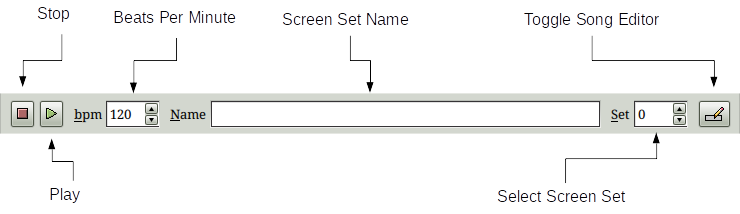
\includegraphics[scale=0.75]{pattern-window-bottom-panel-items.png}
   \caption{Patterns Panel, Bottom Panel Items}
   \label{fig:pattern_window_bottom_panel_items}
\end{figure}

   \begin{enumber}
      \item \textbf{Stop}
      \item \textbf{Play}
      \item \textbf{bpm}
      \item \textbf{Name}
      \item \textbf{Set}
      \item \textbf{Toggle Song Editor}
   \end{enumber}

   \setcounter{ItemCounter}{0}      % Reset the ItemCounter for this list.

   \itempar{Stop}{pattern!stop}
   The red squarebutton stops the playback of the song and all its patterns.
   It is not clear if it also sends MIDI Off messages on all notes.
   \index{keys!esc (stop)}
   The keystroke for stopping playback is the \texttt{Escape} character.

   \itempar{Play}{pattern!Play}
   The green triangular button starts the playback of the whole song.
   \index{keys!space (play)}
   The keystroke for starting playback is the \texttt{Space} character.

   \itempar{bpm}{pattern!bpm}
   The spin widget adjusts the "Beats Per Minute" or BPM value.  The
   range of this field is from 20 bpm to 500 bpm, with a default value of
   120 bpm.
   Although this field looks editable, it is not.  Most keystrokes
   that are entered actually toggle one of the pattern boxes.
   However, the following keys can also modify the BPM in small increments:
   \index{keys!semicolon} The \texttt{semicolon} reduces the BPM;
   \index{keys!apostrophe} The \texttt{apostrophe} increases the BPM.

   \itempar{Name}{pattern!set name}
   Each of the 32 available screen sets can be given a name by entering it
   into this field.

   \textbf{Bug:}
   \index{bugs!set name has side-effect}
   While one is typing in the name of the set in this field, the keystrokes
   will affect the panel window, causing playback to start and pattern
   boxes to be toggled!

   \itempar{Set}{pattern!set number}
   This spin widget selects the current screen set.  The values in this
   field range from 0 to 31, and default to 0.
   Although this field looks editable, it is not.

   \textbf{Bug:}
   \index{bugs!set number has side-effect}
   While one is typing in the number of the set in this field, the keystrokes
   will affect the panel window as well.

   \itempar{Toggle Song Editor}{pattern!toggle song editor}
   Pressing this button toggles the presence on-screen of the Song
   Editor.

%-------------------------------------------------------------------------------
% vim: ts=3 sw=3 et ft=tex
%-------------------------------------------------------------------------------
